\section{Il modello nucleare a goccia}\label{sec:il-modello-nucleare-a-goccia}
Il grafico (Fig.~\ref{fig:en-legame-graph}) della energia di legame media per nucleone commentato in precedenza
contiene un certo numero di importanti indicazioni
sulle proprietà della forza nucleare che sono alla base di un primo
modello del nucleo - suggerito da Bohr nel 1935 - fondato essenzialmente
sul \textbf{raggio finito} della interazione nucleare.
Similmente alle forze intramolecolari a corto raggio nei liquidi,
tale fatto determina una certa analogia tra il comportamento dei nucleoni
nel nucleo e le diverse porzioni di un fluido meccanico incomprimibile, ragione che
giustifica il nome spesso usato di \textbf{modello a goccia}.
\begin{figure}
	\centering
	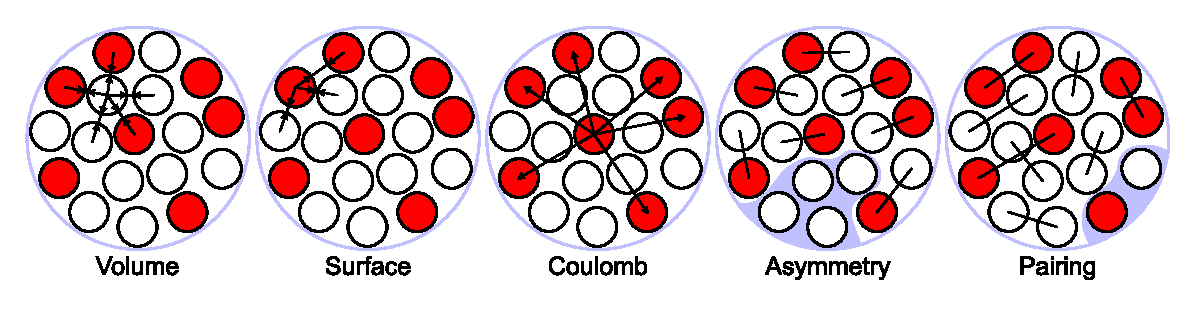
\includegraphics{figs/liquid-drop-model}
	\caption{Rappresentazione grafica del significato fisico dei termini presenti nel nuclear liquid drop model.}
	\label{fig:liquid-drop-model}
\end{figure}

Il suddetto modello ha base \textbf{fenomenologica}; la sola ipotesi
dell'andamento a corto raggio della forza non è sufficiente a
giustificare l'andamento reale

Come accennato, l'energia di legame tende ad assumere rapidamente il
valore medio di circa \(8MeV\) per nucleone (saturazione) il che indica
una energia di legame del nucleo proporzionale al numero di nucleoni
\begin{equation}
	\frac{B}{A} \simeq 8 MeV \qquad B \simeq 8 MeV \times A
    \label{eq:saturation-binding-energy-per-nucleon}
\end{equation}
Ora, se la forza nucleare si comportasse come una forza a lungo
raggio (come le forze gravitazionali o elettromagnetiche) ogni nucleone
interagirebbe con tutti i rimanenti altri per cui dovremmo attenderci
una energia di legame del nucleo tendenzialmente \emph{proporzionale al numero
di coppie} di nucleoni e dunque quadratica in A
\[
	B \propto \frac{A(A-1)}{2} \propto A^{2} \qquad
\]
Poiché i dati sulla energia di legame escludono questo tipo di
comportamento, dobbiamo concludere che ogni nucleone del nucleo
interagisce solo con un numero di fisso di nucleoni vicini per cui
concludiamo che \textbf{l'interazione forte ha un raggio d'azione finito}
dell'ordine di grandezza delle dimensioni del nucleone stesso.

Tale conclusione è in perfetto accordo con i dati sulla sezione d'urto
di neutroni su nuclei analizzati in precedenza che indicavano un \textbf{volume
nucleare proporzionale al numero di nucleoni}, ovvero una densità
volumetrica di nucleoni uniforme sul volume nucleare, fatto spiegabile
solo postulando la esistenza di una forza d'interazione tra nucleoni a
corto raggio.

Il primo tentativo di superare questo limite consiste nell'introdurre un
termine, sulla base della (\ref{eq:saturation-binding-energy-per-nucleon})
\begin{equation}
	B = a_{v} A
   \label{eq:volume-term-drop-model}
\end{equation}
dove la costante \(a_{v}\) viene detta \textbf{termine di volume}.
\begin{marginfigure}
	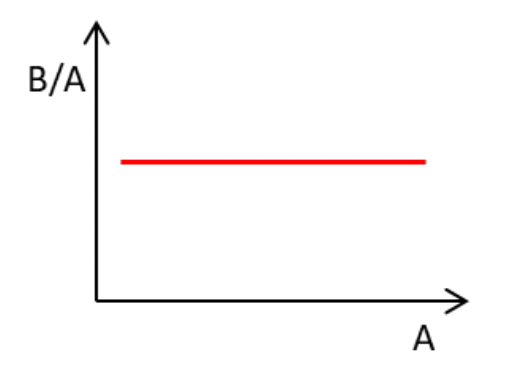
\includegraphics{figs/goccia1}
	%    \caption{This is a margin figure.}
	\label{fig:goccia1}
\end{marginfigure}
Con un tale andamento \(B / A\) , però, si finisce per ottenere una sovrastima
del volume.
La deviazione più rilevante si manifesta per valori piccoli di A dove
l'energia media di legame è molto inferiore a quanto previsto dalla
formula.
\bigskip

Si può allora osservare che, assumendo la forza nucleare a
corto raggio, si deve tenere conto che un nucleone prossimo alla
superficie del nucleo interagirà con un numero di nucleoni inferiore a
quello con cui interagirebbe qualora si trovasse all'interno del nucleo
stesso.
Ciò comporta che i nucleoni superficiali contribuiranno in
misura minore alla energia di legame nucleare di quelli interni al
volume.
Assumendo il nucleo di \textbf{forma sferica}, il numero di
nucleoni prossimi alla superficie sarà proporzionale a \(R^{2}\).
Dalla trattazione precedente (\ref{eq:nuclear-radius-skin}) sappiamo che (omettendo il termine di `skin'
nucleare) \begin{gather*}
	R_{\text{nuc}} = r_{0}A^{1/3}\\
	4 \pi R^{2} = 4 \pi (r_{0}A^{1/3})^2 \implies R_{\text{nuc}} \propto A^{2/3}
\end{gather*} per cui vi deve essere un termine che deve provocare un difetto di
energia di legame proporzionale ad \(A^{2/3}\): \[
	B = a_{v}A - a_{s}A^{2/3}
\] dove la costante \(a_{s}\) viene detta \textbf{termine di
	superficie}.
L'andamento di \(B / A\) con questa ulteriore correzione
può apprezzarsi a lato.
\begin{marginfigure}
	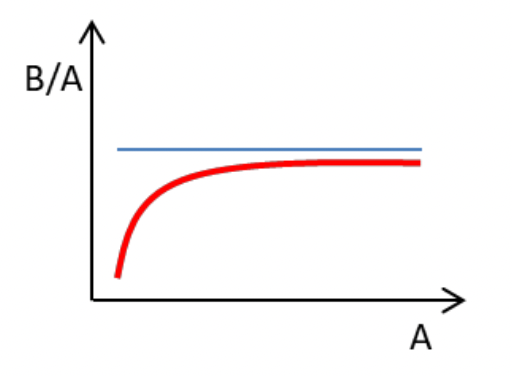
\includegraphics{figs/goccia2}
	%    \caption{This is a margin figure.}
	\label{fig:goccia2}
\end{marginfigure}
\bigskip

Un ulteriore miglioramento può essere ottenuto tenendo presente che i
protoni del nucleo si \emph{respingono elettrostaticamente} diminuendo
quindi il lavoro necessario per separarli dal nucleo stesso.
In effetti
se, per assurdo, si avesse un nucleo composto solo di protoni(senza
neutroni) il lavoro da spendere per mantenerne la configurazione sarebbe
sicuramente maggiore.

Ipotizzando una \emph{distribuzione di protoni uniforme} nel volume
nucleare (ricordiamo essere sferico dall'ipotesi precedente), otteniamo
la seguente espressione del lavoro fatto dalle forze coulombiane
repulsive per separare la carica nucleare
\begin{gather*}
	\delta L = \int _{R}^{\infty} \left( \frac{q \delta q}{4 \pi \epsilon_{0}r^{2}}  \hat{\bm{r}} \right)(dr \hat{\bm{r}})=
	- \frac{q \delta q}{4 \pi \epsilon_{0}r} \bigg |_{R}^{\infty} =
	- \frac{q \delta q}{4 \pi \epsilon_{0}R}\\
	q = \rho \frac{ 4}{3} \pi R^{3} \qquad \delta q = \rho 4 \pi R^{2} dR\\
	\delta L = \frac{1}{4 \pi \epsilon_{0}R}\left( \rho \frac{ 4}{3}\pi R^{3} \right)(\rho 4 \pi R^{2} dR) = \frac{4 \pi \rho^{2}}{3 \epsilon_{0}}R^{4}dR\\
	L = \int \delta l = \frac{4 \pi \rho^{2}}{15 \epsilon_{0}}R_{0}^{5} \qquad Q = \rho \frac{ 4}{3} \pi R_{0}^{3} = Ze\\
	L = \frac{3}{20 \pi \epsilon_{0}} \frac{Q^{2}}{R_{0}} = \frac{3e^{2}}{20 \pi \epsilon_{0}r_{0}} \frac{Z^{2}}{A^{1/3}}
	\implies L \propto \frac{ Z^{2}}{A^{1/3}}
\end{gather*} Ne consegue che la energia di legame nucleare dovrà essere corretta
sottraendo un termine proporzionale a \(Z^{2} / A^{1/3}\) per cui
l'espressione dell'energia di legame acquisirà la forma seguente
\begin{equation}
	B = a_{v}A - a_{s}A^{2/3} - a_{c} \frac{Z^{2}}{A^{1/3}}
	\label{eq:coulomb-term-drop-model}
\end{equation}
 dove la nuova costante \(a_{c}\) viene detta \textbf{termine
	coulombiano}.
Il termine coulombiano deve chiaramente annullarsi per
\(A=1\)(non c'e interazione elettrostatica) per cui l'unica forma
possibile è \[
	L \propto \frac{Z(Z-1)}{A^{1/3}} \quad
\]
\begin{marginfigure}
	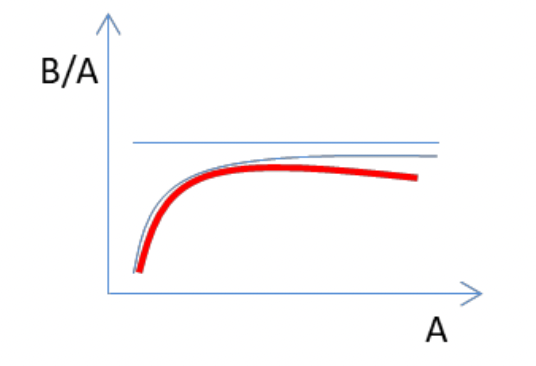
\includegraphics{figs/goccia3}
	%    \caption{This is a margin figure.}
	\label{fig:goccia3}
\end{marginfigure}

L'andamento $B / A$ risulta ulteriormente migliorato (si tenga presente
che nei nuclei stabili si ha approssimativamente \(Z=A/2\) per cui il
termine coulombiano sottrae un contributo crescente con \(A^{5/3}\)).

Se il modellino fenomenologico costruito finora fosse completo dovremmo
concludere che i nuclei più stabili(\(B= B_{max}\)) sono quelli con
\(Z=0\) ovvero i nuclei di soli neutroni.
Tale fatto è palesemente
contraddetto dai dati sperimentali i quali mostrano che i nuclei stabili
hanno un numero di protoni di poco inferiore a quello dei neutroni (la
differenza tra neutroni e protoni tende a crescere con il numero
atomico).
Il nostro modello -- basato sulla natura a corto raggio della
interazione nucleare -- non offre alcun appiglio per dare un fondamento
fisico a questo stato di cose che potrà essere spiegato solo nel
contesto della meccanica quantistica attraverso il \emph{principio di
	esclusione di Pauli}.
In questa situazione l'unica possibilità è quella
di introdurre un termine `ad hoc' capace di descrivere i dati
sperimentali.

Bisogna quindi fare in modo che il modello ci dica che i nuclei piu
stabili sono quelli con lo stesso numero di protoni e neutroni.
Raggiungiamo l'obiettivo introducendo un nuovo termine del tipo:
\[
	Z \simeq \frac{A}{2} \quad A - 2Z \simeq 0
\]
Ricordando però che con il crescere di \(A, Z\) tende ad essere via
via più piccolo di \(A/2\) (il quoziente protoni/neutroni diminuisce con
\(A\)), tale termine correttivo dovrà seguire una legge inversa ad A
modulata da un qualche esponente.
I dati indicano che la prima potenza è
sufficiente per cui abbiamo la seguente espressione della energia di
legame nucleare
\[
	B = a_{v}A - a_{s}A^{2/3} - a_{c} \frac{Z(Z-1)}{A^{1/3}} - \frac{a_{a}(A-2Z)^{2}}{A}
\]
dove la nuova costante \(a_{a}\) viene detta \textbf{termine di asimmetria}.
Notiamo che la presenza di \(A\) a denominatore è
giustificata osservando l'andamento dei dati sperimentali nel grafico
visto in precedenza:tanto piu \(A\) è grande tanto piu \(B / A\) devia
dalla tangente alla curva (quindi verso il basso).

Per completare il modello è necessario tenere conto di un ulteriore
proprietà dei nuclei.
I dati sperimentali mostrano che tra i 254 nuclei
stabili noti ben 148 sono del tipo \textbf{pari-pari} (un numero pari
sia di protoni che di neutroni), 101 sono del tipo \textbf{pari-dispari}
(un numero pari di protoni ma dispari di neutroni o viceversa) e solo 5
sono del tipo dispari-dispari (riportati in tabella \ref{tab:odd-odd-stable-nuclei}).
\begin{table}
	\centering
	\begin{tabular}{|c|}
		\hline
		$\isotope[2][1]{\mathlarger{H}}$ \\ \hline
		$\isotope[6][3]{\mathlarger{Li}}$ \\ \hline
		$\isotope[10][5]{\mathlarger{B}}$ \\ \hline
		$\isotope[14][7]{\mathlarger{N}}$ \\ \hline
		$\isotope[180m][73]{\mathlarger{Ta}}$ \\ \hline
	\end{tabular}
	\caption{Tabella dei nuclei stabili con both $ A,Z$ dispari. L'$m$ ad apice indica la metastabilità del nuclide. \\
	Si veda \url{https://en.wikipedia.org/wiki/Metastability#Nuclear_physics} a tale proposito.}
	\label{tab:odd-odd-stable-nuclei}
\end{table}

Similmente, tra i 35 nuclei a lunga vita media si hanno 22 pari-pari, 9 pari-dispari e 4
dispari-dispari.

Tali dati sembrano suggerire che per qualche motivo la forza forte tra
nucleoni da luogo a nuclei di maggiore stabilità quando vengono legati
\textbf{numeri pari} di neutroni e protoni, un fatto che trova una sua
diretta evidenza nell'andamento della energia di legame per nucleone
della serie isotopica dello xenon in Figura~\ref{fig:binding-energy-xenon}.
Tali dati sembrano suggerire che per qualche motivo la forza forte tra nucleoni da luogo a nuclei di maggiore stabilità
quando vengono legati \textbf{numeri pari} di neutroni e protoni, un fatto che trova una sua diretta evidenza nell’andamento della energia di legame per nucleone della serie isotopica dello xenon.
\begin{marginfigure}
	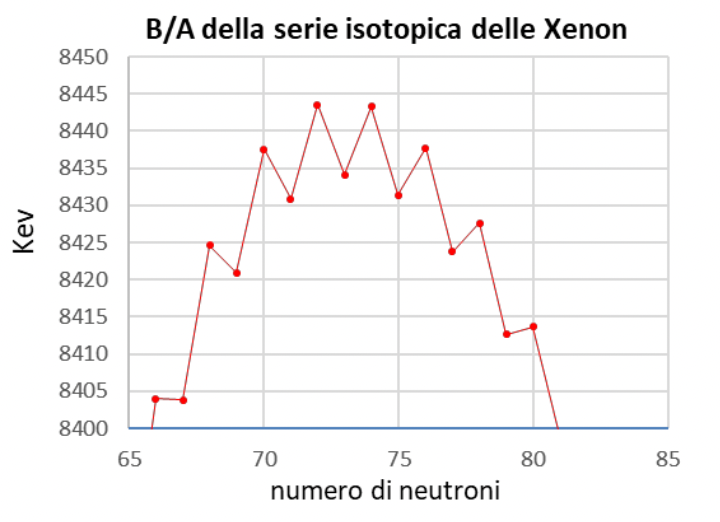
\includegraphics[scale = 1.5]{figs/goccia5}
	\caption{Andamento dell'energia di legame per la serie isotopica dello Xenon.}
	\label{fig:binding-energy-xenon}
\end{marginfigure}
Tenendo presente che il nucleo di Xenon ha \(Z=54\) protoni, si può
infatti constatare che gli isotopi con un numero pari di neutroni hanno
una maggiore energia di legame per nucleone.
Per rendere conto di questo
fatto si introduce un nuovo coefficiente detto di \textbf{pairing} \[
	a_{p} \frac{\delta}{A^{3/4}}
\] con \[
	\delta =
	\begin{cases}
		+1    \qquad  \text{pari-pari}       \\
		\ 0  \qquad  \ \ \text{pari-dispari} \\
		-1  \qquad  \text{dispari-dispari}
	\end{cases}
\] Giungiamo così alla seguente espressione complessiva della energia di
legame nucleare detta anche \textbf{formula semiempirica della energia
	di legame nucleare} o \textbf{formula di Weizsacker} della energia di
legame nucleare
\begin{equation}
	\boxed{    B = a_{v}A - a_{s}A^{2/3} - a_{c} \frac{Z(Z-1)}{A^{1/3}} - a_{a}\frac{(A-2Z)^{2}}{A} +     a_{p} \frac{\delta}{A^{3/4}}}
	\label{eq:weizsacker-formula}
\end{equation} Essa dipende da 5 parametri(vedi Fig.~\ref{fig:liquid-drop-model}) il cui valore numerico
viene determinato adattando la formula ai dati sperimentali di \(B/A\).

A titolo di esempio, una possibile combinazione di valori è la seguente(i
valori sono in \(MeV\)):
\[
	a_{v} = 15.5 \quad a_{s} = 16.8 \quad a_{c} = 0.72 \quad a_{a} = 23.0 \quad a_{p} = 34.0
\]
La formula della energia di legame nucleare è utile - come strumento di
calcolo - perchè suggerisce una prima interpretazione del nucleo e delle
forze che lo tengono insieme.

Da essa deduciamo che le forze tra nucleoni devono essere \textbf{molto
	intense} ma a \textbf{short range} (proprietà di saturazione), producono
una distribuzione spaziale tendenzialmente uniforme di nucleoni e
conducono ad una espressione della energia di legame con termini di
volume e superficie in analogia con quanto accade per i liquidi, ragione
che giustifica il nome spesso usato di \textbf{modello nucleare a
	goccia}.

Il \emph{modello a gas di fermioni} (giustificabile con considerazioni
quantomeccaniche) riesce a rendere conto del termine \(a_{a}\) mentre
fallisce per quello di pairing.
Vedremo, infine, che il \emph{modello a shell} sarà quello piu preciso.

%%%%%%%%%%%%%%%%%%%%%%%%%%%%%%%%%%%%%%%%%%%%%%%%%%%%%%%%%%%%%%%%%%%%%%%%%%%%%%%%%%%%%%%%%%%%%%%%%%%%%%%%%%%%%%%%%%%%%%%%
%%%%%%%%%%%%%%%%%%%%%%%%%%%%%%%%%%%%%%%%%%%%%%%%%%%%%%%%%%%%%%%%%%%%%%%%%%%%%%%%%%%%%%%%%%%%%%%%%%%%%%%%%%%%%%%%%%%%%%%%
%%%%%%%%%%%%%%%%%%%%%%%%%%%%%%%%%%%%%%%%%%%%%%%%%%%%%%%%%%%%%%%%%%%%%%%%%%%%%%%%%%%%%%%%%%%%%%%%%%%%%%%%%%%%%%%%%%%%%%%%
\section{Il nucleo come gas di fermioni}\label{sec:il-nucleo-come-gas-di-fermioni}

Il modello a goccia del nucleo - essenzialmente fondato sulla natura a corto raggio delle interazioni forti - riesce a
descrivere alcune proprietà del nucleo tra le quali l’esistenza di una energia di legame con termini di volume, superficie e coulombiano.
Non riesce invece a rendere conto in nessun modo dei termini di asimmetria e accoppiamento, chiaramente richiesti dai
dati sperimentali, ma che devono essere introdotti ‘a mano’ nella formula di Weizsacker.
Tale fatto dimostra che oltre alla natura a corto raggio delle interazioni forti, nel nucleo giocano un ruolo di rilievo
altre proprietà trascurate dal modello a goccia, presumibilmente legate alla natura quantomeccanica dei suoi costituenti.
Il modello nucleare a gas di fermioni introduce nel gioco alcuni essenziali proprietà quantomeccaniche in una forma il
più possibile semplificata.





